\section{Theorie}
\label{sec:Theorie}
In einem Kristallgitter, welches aus einfach geladenen Ionen besteht, werden einzelne dieser Ionen durch zweiwertige ersetzt.
Wegen der elektrischen Ladungsneutralität eines Kristalls entstehen Leerstellen (vgl. Abbildung \ref{fig:t:2}.
%%%%%%%%%%%%%%%%%%%%%%%%%%%
\begin{figure}
\centering
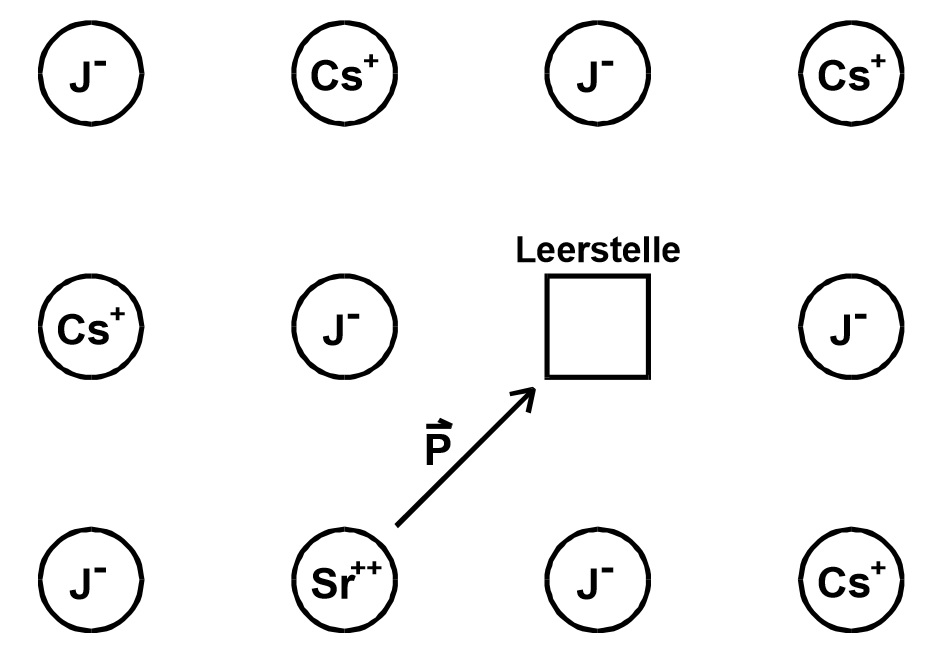
\includegraphics[scale=0.5]{content/kristall.jpg}
\caption{Entstehung von Dipolen in einem Caesium-Iod Kristall durch hinzufügen von Strontium Ionen \cite{Anleitung}.}
\label{fig:t:2}
\end{figure}
%%%%%%%%%%%%%%%%%%%%%%%%%%%%%%
Zusammen mit den zweiwertigen Ionen bilden die Leerstellen Dipole, deren Verhalten im folgenden untersucht werden soll.
Bei den Temperaturen, die bei diesen Untersuchungen erreicht werden, bewegen sich im Kristall hauptsächlich die zweiwertigen Ionen.
Um eine neue Position im Gitter einzunehmen, muss eine Potential Barriere überwunden werden.
Die dadurch bestimmte Energie ist die Aktivierungsenergie $W$.
Aus statistischen Überlegungen lässt sich der Anteil der Ionen, die diese Energie besitzen, als 
\begin{align}
\exp \left(\frac{-W}{kT}\right)
\label{eq:t:1}
\end{align}
bestimmen.
Ebenso folgt die Relaxationszeit
\begin{align}
\tau(T)=\tau_0 \exp\left(\frac{W}{kT}\right)\text{ ,}
\label{eq:t:2}
\end{align}
welche die mittlere Zeit zwischen zwei Positionswechseln beschreibt.

\noindent
Durch Anlegen eines elektrischen Feldes lassen sich die Dipole in eine Vorzugsrichtung ausrichten.
Dabei ist zu beachten, dass aufgrund der thermischen Bewegungen nur ein bestimmter Anteil $y$ aller Dipole in diese Richtung weist.
Dieser Anteil ist durch die Langevin-Funktion 
\begin{align}
y=L(x)=\cot (x) -\frac{1}{x}
\label{eq:t:3}
\end{align}
gegeben, wobei $x=\frac{pE}{kT}$ gewählt wird.
Da unter den folgenden Messbedingungen $pE<<kT$ gilt, kann $y$ durch
\begin{align}
y(T)=\frac{pE}{3kT}
\label{eq:t:4}
\end{align}
genährt werden.
Die hier gewählte Messmethode erfordert ein Abkühlen der Probe, um den durch das elektrische Feld erzeugten Zustand einzufrieren.
Durch Aufheizen der Probe können mit den im folgenden beschriebenen Methoden die Aktivierungsenergie $W$ und die Konstante $\tau_0$ aus Formel (\ref{eq:t:2}) bestimmt werden. 
Um die Rechnung zu vereinfachen wird eine konstante Heizrate
\begin{align}
b=\frac{dT}{dt}=\text{const}
\label{eq:t:5}
\end{align}
angenommen.
Das Aufheizen der Probe und die damit verknüpfte wachsende thermische Energie des Kristallgitters führt zu einer wachsenden Anzahl an Dipolen, die aus der Vorzugsrichtung herausspringen können.
In einem externen Stromkreis kann daher ein Depolarisationsstrom gemessen werden. 
Die Depolarisationsstromdichte $j$ hängt von der Gesamtpolarisation, der Anzahl der Dipole in Vorzugsrichtung bei der Polarisationstemperatur $T_p$ und der Änderung der Dipole in Vorzugsrichtung ab
\begin{align}
j(T)=y(T_p)~p~\frac{dN}{dt} \overset{Gl. (\ref{eq:t:4})}{=} \frac{p^2E}{rkT_p}\frac{dN}{dt}\text{ .}
\label{eq:t:6}
\end{align}
Die Anzahl der relaxierenden Dipole ist proportional zur Anzahl der ausgerichteten Dipole
\begin{align}
\frac{dN}{dt}=-\frac{N}{\tau(T)} \text{ .}
\label{eq:t:7}
\end{align}
Daraus ergibt sich unter dem Einfluss der konstanten Heizrate
\begin{align}
N=N_p\exp \left(-\frac{1}{b} \int_{T_0}^T \frac{dT\prime}{\tau(T\prime)}\right) \text{ .}
\label{eq:t:8}
\end{align}
Zusammen mit den Gleichungen (\ref{eq:t:4}) und (\ref{eq:t:6}) folgt für die Depolarisationsstromdichte
\begin{align}
j(T)=\frac{p^2E}{3kT}\frac{N_p}{\tau_0}\exp \left(-\frac{W}{kT}\right)\exp\left(-\frac{1}{b\tau_0}\int_{T_0}^T\exp\left(-\frac{W}{kT}\right)dT\prime\right) \text{ .}
\label{eq:t:9}
\end{align}
Wird für den Anfangsbereich zusätzlich die Näherung 
\begin{align}
\int_{T_0}^T\exp\left(-\frac{W}{kT}\right)dT\prime\approx 0	
\label{eq:10}
\end{align}
angenommen, folgt aus Gleichung (\ref{eq:t:6}) 
\begin{align}
j(T)=\frac{p^2E}{3kT}\frac{N_p}{\tau_0}\exp \left(-\frac{W}{kT}\right)\text{ .}
\label{eq:t:11}
\end{align}
Abbildung \ref{fig:t:1} zeigt skizzenhaft den Kurvenverlauf des Depolarisationsstroms nach dieser Gleichung.
%%%%%%%%%%%%%%%%%%%%%%%%%%%
\begin{figure}
\centering
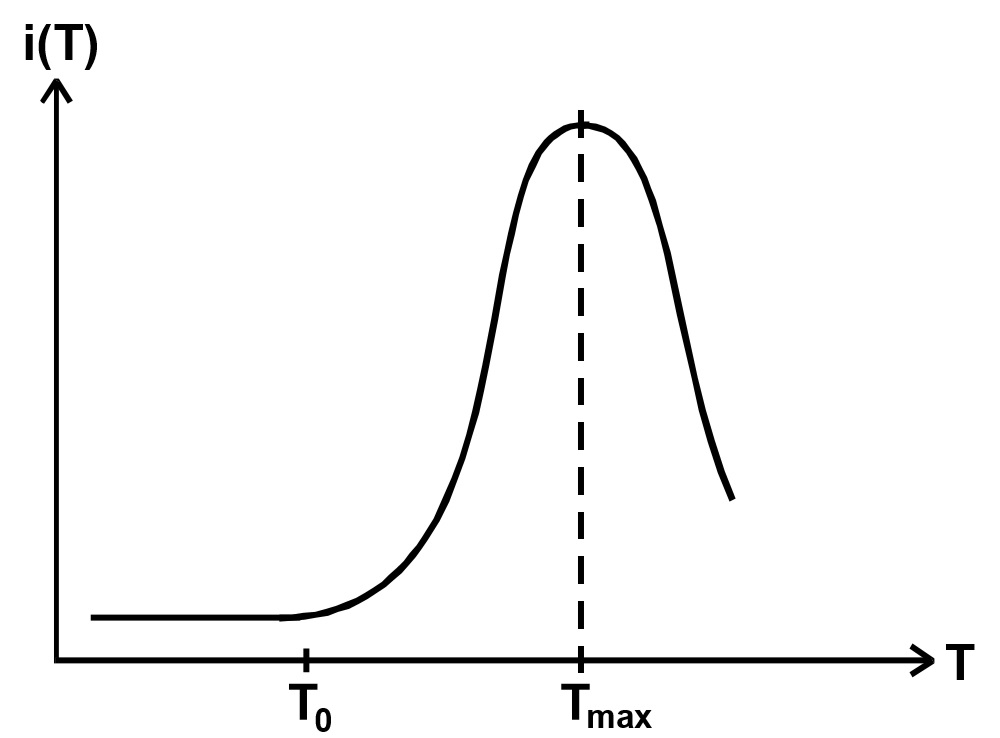
\includegraphics[scale=0.5]{content/kurve.jpg}
\caption{Mit steigender Temperatur relaxieren die Dipole. Da die Anzahl der noch nicht relaxierten Dipole deshalb stetig abnimmt fällt die Steigung der Kurve mit zunehmender Temperatur wieder ab und die Kurve erreicht ein Maximum \cite{Anleitung}.}
\label{fig:t:1}
\end{figure}
%%%%%%%%%%%%%%%%%%%%%%%%%%%%%%
Mithilfe der Polarisation $P$ lässt sich eine Methode die Aktivierungsenergie $W$ zu bestimmen entwickeln, die sich nicht auf den Anfangsbereich der Kurve beschränkt, sondern den gesamten Kurvenverlauf berücksichtigt.
Die Änderung der Polarisation ist proportional zur Anzahl der ausgerichteten Dipole
\begin{align}
\frac{dP}{dt}=-\frac{P(t)}{\tau(T(t))}\text{ .}
\label{eq:t:12}
\end{align}
Die für den durch die Depolarisation entstehenden Strom geltende Gleichung
\begin{align}
i(t)=F\frac{dP}{dt}\text{ ,}
\label{eq:t:13}
\end{align}
wobei $F$ den Querschnitt der Probe bezeichnet, lässt sich einfach integrieren und mit Gleichung (\ref{eq:t:12}) kombinieren.
Zusammen folgt
\begin{align}
\tau(T(t))=\frac{1}{i(t(T))}\int_{t(T)}^\infty i(t)dt \text{ .}
\label{eq:t:14}
\end{align}
Zuletzt lässt sich Gleichung (\ref{eq:t:14}) durch die Annahme der konstanten Heizrate zu
\begin{align}
\frac{W}{kT}=\log\left(\frac{1}{i(T)b\tau_0}\int_T^\infty i(T\prime)dT\prime\right)
\label{eq:t:15}
\end{align}
vereinfachen.
Die Aktivierungsenergie lässt sich so direkt aus der Steigung einer Ausgleichsgeraden ablesen.
Um den Zusammenhang zwischen der Relaxationszeit und der Temperatur zu beschreiben muss noch die Größe $\tau_0=\tau(\infty)$ aus Gleichung (\ref{eq:t:2}) bestimmt werden. 
Diese lässt sich aus der Lage des Strommaximums berechnen (vgl. Abbildung \ref{fig:t:1}).
Dazu wird Gleichung (\ref{eq:t:9}) nach $T$ abgeleitet
\begin{align*}
\frac{d}{dT}j(T)&=\frac{p^2E}{3kT_p}\frac{N_p}{\tau_0}\exp\left(-\frac{1}{b\tau_0}\int_{T_0}^T\exp\left(-\frac{W}{kT}\right)dT\prime\right)\frac{d}{dT}\left(\exp \left(-\frac{W}{kT}\right)\right)\\
&+\frac{p^2E}{3kT}\frac{N_p}{\tau_0}\exp \left(-\frac{W}{kT}\right)\frac{d}{dT}\left(\exp\left(-\frac{1}{b\tau_0}\int_{T_0}^T\exp\left(-\frac{W}{kT}\right)dT\prime\right)\right)\\
&=\frac{p^2E}{3kT_p}\frac{N_p}{\tau_0}\exp\left(-\frac{1}{b\tau_0}\int_{T_0}^T\exp\left(-\frac{W}{kT}\right)dT\prime\right)\left(\frac{W}{kT^2}\right)\exp\left(-\frac{W}{kT}\right)\\
&+\frac{p^2E}{3kT}\frac{N_p}{\tau_0}\exp \left(-\frac{W}{kT}\right)\left(\exp\left(-\frac{W}{kT}\right)-\exp\left(-\frac{W}{kT_0}\right)\right)\exp\left(-\frac{1}{b\tau_0}\int_{T_0}^T\exp\left(-\frac{W}{kT}\right)dT\prime\right)\\ \text{ .}
\end{align*}
Daraus folgt für das Extremum
\begin{align*}
\frac{d}{dT}j(T)=0 \Longrightarrow -\frac{1}{b\tau_0}\left(\exp\left(-\frac{W}{kT_\text{max}}\right)-\exp\left(-\frac{W}{kT_0}\right)\right)+\frac{W}{kT_\text{max}^2}=0 \text{ .}
\end{align*}
Insgesamt gilt also
\begin{align}
\tau_0=\frac{kT_\text{max}^2}{Wb}\left(\exp\left(-\frac{W}{kT_\text{max}}\right)-\exp\left(-\frac{W}{kT_0}\right)\right)  \text{ .}
\label{eq:t:16}
\end{align}